\newpage
\section{Rectificador de precisión}
\onehalfspacing
\begin{figure}[htb]
	\centering
	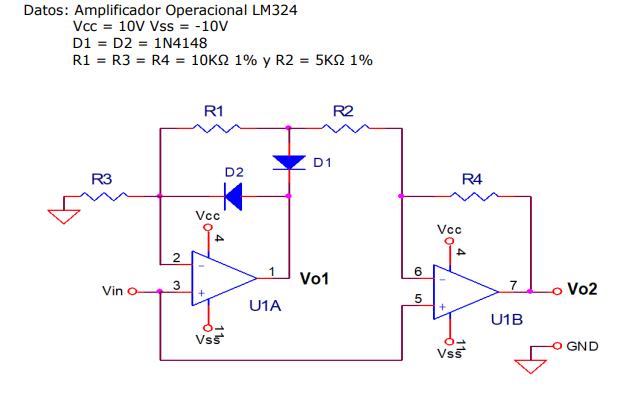
\includegraphics[width=1\textwidth]{figuras/Circuito3_consigna.png}
	\caption{Circuito propuesto}
\end{figure}
En este circuito se tienen 2 AO LM324 con diodos trabajando como un rectificador de precisión con una señal común para ambos. La fuente de alimentación es simétrica en +/- 10[V]. Los diodos utilizados son 1N4148.
\subsection{Análisis teórico}
Para determinar $V_o$ en función de $V_{in}$ el análisis se hace para cuando $V_{in}$ es positiva y cuando $V_{in}$ es negativa.
\subsubsection{$V_o = f(V_{in})$ con $V_{in}$ $> 0$  }
Para ésta condición entonces D2 = ON y D1= OFF. \\
Además considerando pasivada la entrada del AO U1B se plantea la ley de los nodos de Kirchhoff en el nodo "6"
\begin{center}
	$\frac{V_o}{R_4} = - \frac{V_{in}}{R_1 + R_2}$
\end{center}
\begin{center}
	$\frac{V_o}{10[K\Omega]} = - \frac{V_{in}}{15[K\Omega]}$
\end{center}
\begin{center}
	$V_o= - \frac{2}{3} V_{in}$
\end{center}
Luego pasivando la entrada de U1A
\begin{center}
	$V_{in}= V_o \frac{R_1 + R_2}{R_1 + R_2 + R_4}$
\end{center}
\begin{center}
	$V_{in}= V_o \frac{15[K\Omega]}{25[K\Omega]}$
\end{center}
\begin{center}
	$V_o = \frac{5}{3} V_{in}$
\end{center}
Aplicando superposición para encontrar el resultado completo
\begin{center}
	$V_o = V_{in} \frac{5}{3} - V_{in} \frac{2}{3}$
\end{center}
\begin{center}
	\boxed{V_o = V_{in} }
\end{center}

\subsubsection{$V_o = f(V_{in})$ con $V_{in}$ $< 0$  }
Para ésta condición entonces D1 = ON y D2= OFF. \\
Además considerando pasivada la salida del AO U1A se plantea la ley de los nodos de Kirchhoff en el nodo "6"
\begin{center}
	$V_{in} = V_o \frac{R_2}{R_2 + R_4}$
\end{center}
\begin{center}
	$V_{in} = V_o \frac{5[K\Omega]}{15[K\Omega]}$
\end{center}
\begin{center}
	$V_o= 3 V_{in}$
\end{center}
Luego pasivando la entrada de U1B y tomando $V_{oB}$ como tensión de salida del amplificador U1B, resulta:
\begin{center}
	$\frac{V_{oB}}{R_2} =- \frac{V_o}{R_4}$
\end{center}
\begin{center}
	$\frac{V_{oB}}{5[K\Omega]} =- \frac{V_o}{10K\Omega}$
\end{center}
\begin{center}
	$V_o = -2 V_{oB} $
\end{center}
Por otro lado, la tensión de salida de $V_{oB}$ se obtiene planteando el divisor de tension del AO U1B:
\begin{center}
	$V_{in} = V_{oB} \frac{R_3}{R_1 + R_3}$
\end{center}
\begin{center}
	$V_{in} = V_{oB} \frac{10K\Omega}{20K\Omega}$
\end{center}
\begin{center}
	$V_{in} =\frac{1}{2} V_{oB} $
\end{center}
Reemplazando queda:
\begin{center}
	$V_o = -4 V_{in} $
\end{center}
Aplicando superposición para encontrar el resultado completo
\begin{center}
	$V_o = 3 V_{in} - 4 V_{in}$
\end{center}
\begin{center}
	\boxed{V_o = - V_{in} }
\end{center}
Entonces, cuando la tensión de entrada es positiva, la tensión de salida es igual a la entrada, mientras que cuando la tensión de entrada es negativa, la tensión de salida tendrá la misma amplitud pero será positiva.
\subsection{Simulación}
Se realizaron diferentes simulaciones con LTSpice para observar el comportamiento a la salida para diferentes valores de entrada. Primero se hizo un DC sweep con valores de $V_{in}$ que van desde -10[V] a los 10[V]. Luego se realizó un Trasient con frecuencia de 1[KHz].
\begin{figure}[H]
	\centering
	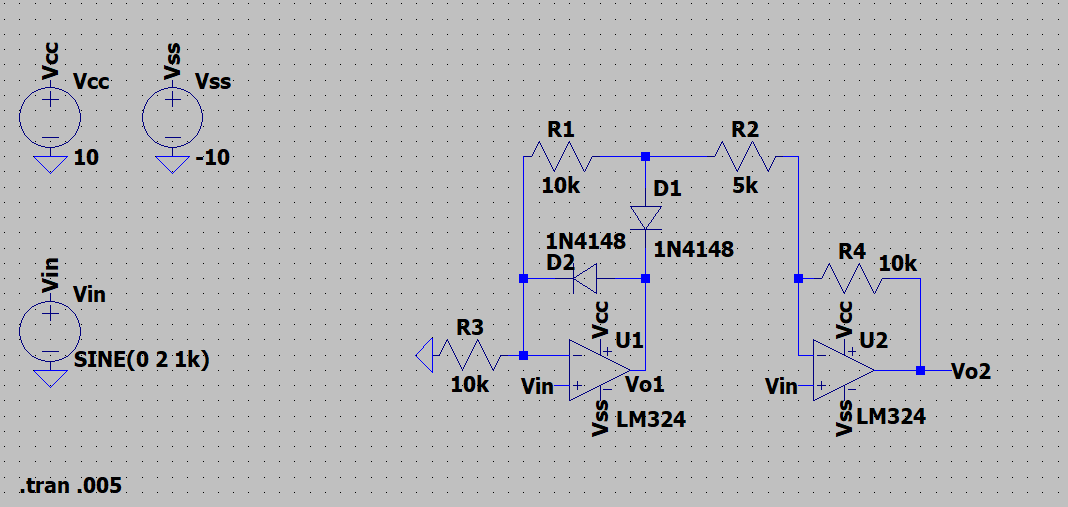
\includegraphics[width=1\textwidth]{figuras/Circuito3.png}
	\caption{Circuito simulado}
\end{figure}
\begin{figure}[H]
	\centering
	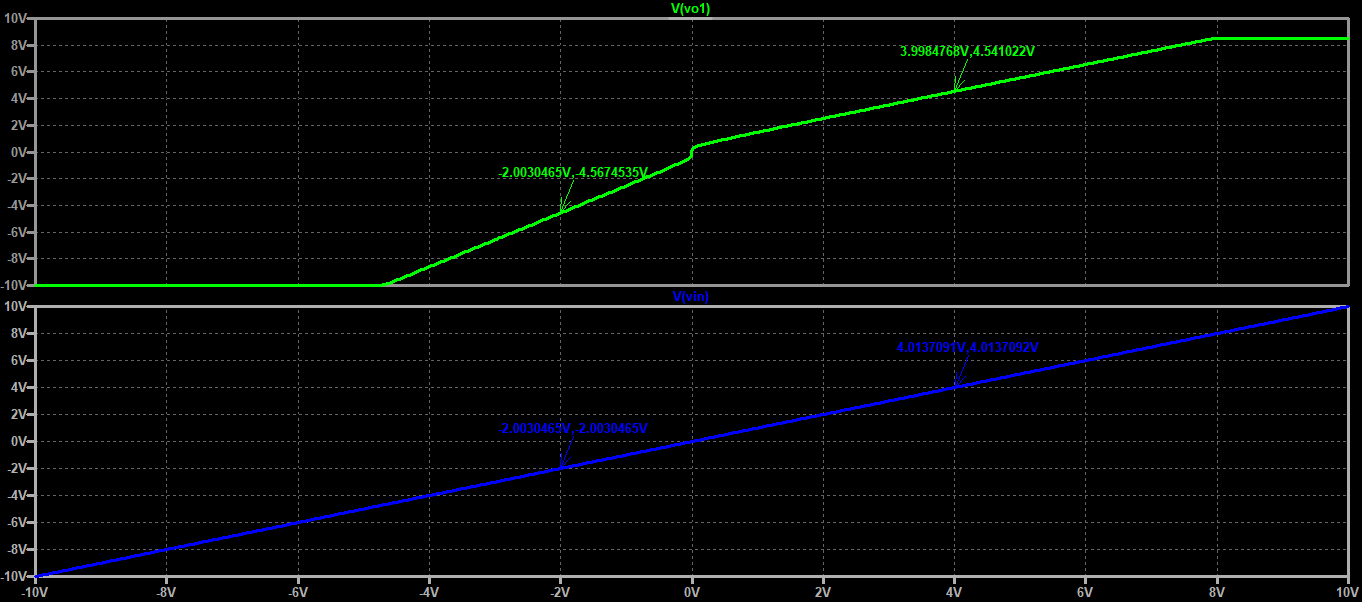
\includegraphics[width=1\textwidth]{figuras/dc_sweep_vo1.png}
	\caption{Dc sweep $Vo_1$ (verde) $ -10[V] < V_{in} < 10 [V]$(azul).}
\end{figure}
Como se observa en los puntos marcados, la salida es duplicada para valores negativos de entrada mientras que para valores positivos de entrada, son copiados a la salida.
También para baja excursión presenta alta ganancia y alinealidades.
\begin{figure}[H]
	\centering
	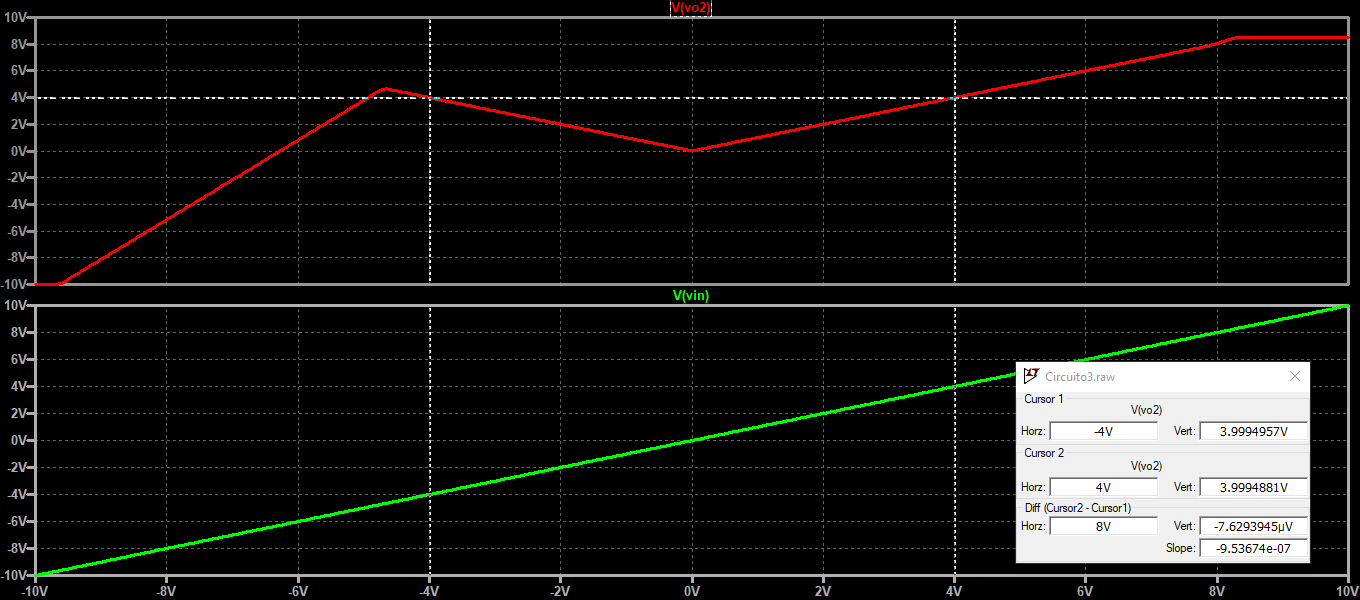
\includegraphics[width=1\textwidth]{figuras/dc_sweep_vo2.png}
	\caption{Dc sweep $Vo_2$ (rojo) $ -10[V] < V_{in} < 10 [V]$ (verde).}
\end{figure}
Como se observa  en el rango de -4[V] a 4[V] la salida es el valor absoluto del valor de la entrada, es decir una rectificación completa de una onda senoidal.\\
A continuación las simulaciones Transient con $V_{in}$ variable y de frecuencia 1[KHz].

\begin{figure}[H]
	\centering
	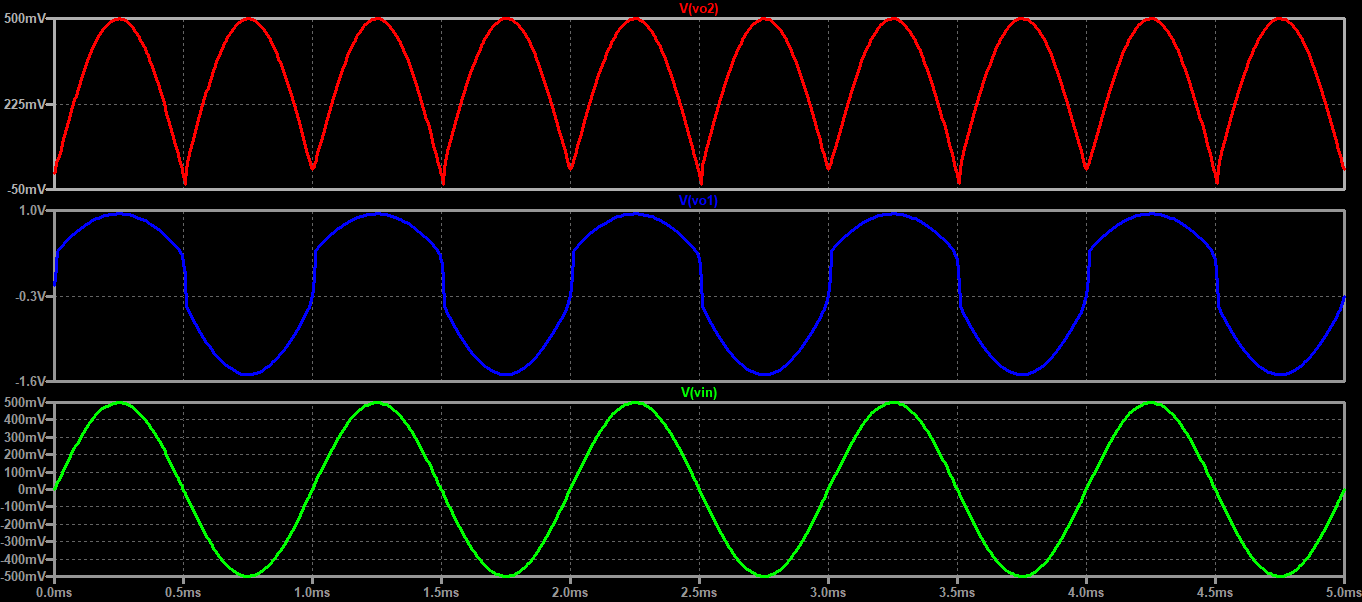
\includegraphics[width=1\textwidth]{figuras/Vo1_Vo2_Vin=0.5.png}
	\caption{$Vo_1$ (azul) y $Vo_2$ (rojo) con $V_{in}=0.5[V]$.}
\end{figure}
\begin{center}
	\begin{tabular}{| c | c |}
		\hline
				& $V_{in}= 0.5[V]$ \\ \hline
		$Vo_1$ 	&  	947.31 [mV]	 \\
		$Vo_2$ 	& 	498.53 [mV]	 \\ \hline
	\end{tabular}
\end{center}
\begin{figure}[H]
	\centering
	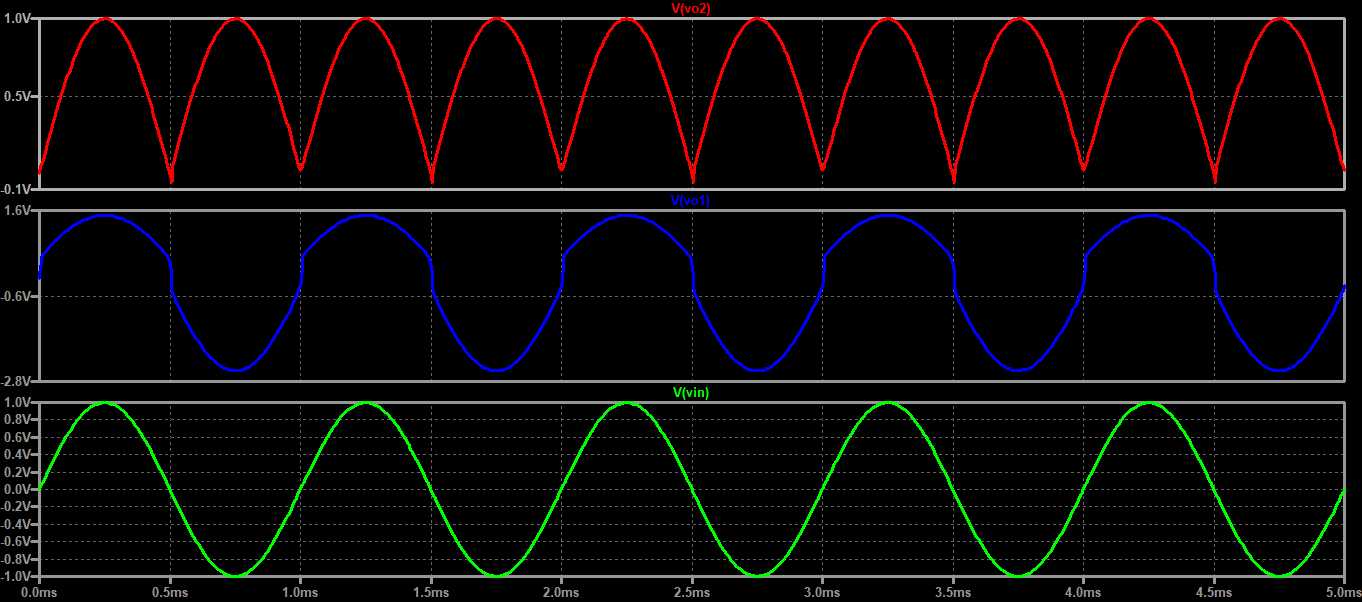
\includegraphics[width=1\textwidth]{figuras/Vo1_Vo2_Vin=1.png}
	\caption{$Vo_1$ (azul) y $Vo_2$ (rojo) con $V_{in}=1[V]$.}
\end{figure}
\begin{center}
	\begin{tabular}{| c | c |}
		\hline
		& $V_{in}= 1[V]$ \\ \hline
		$Vo_1$ 	&  	  1.47 [V]	 \\
		$Vo_2$ 	& 	997.73 [mV]	 \\ \hline
	\end{tabular}
\end{center}
\begin{figure}[H]
	\centering
	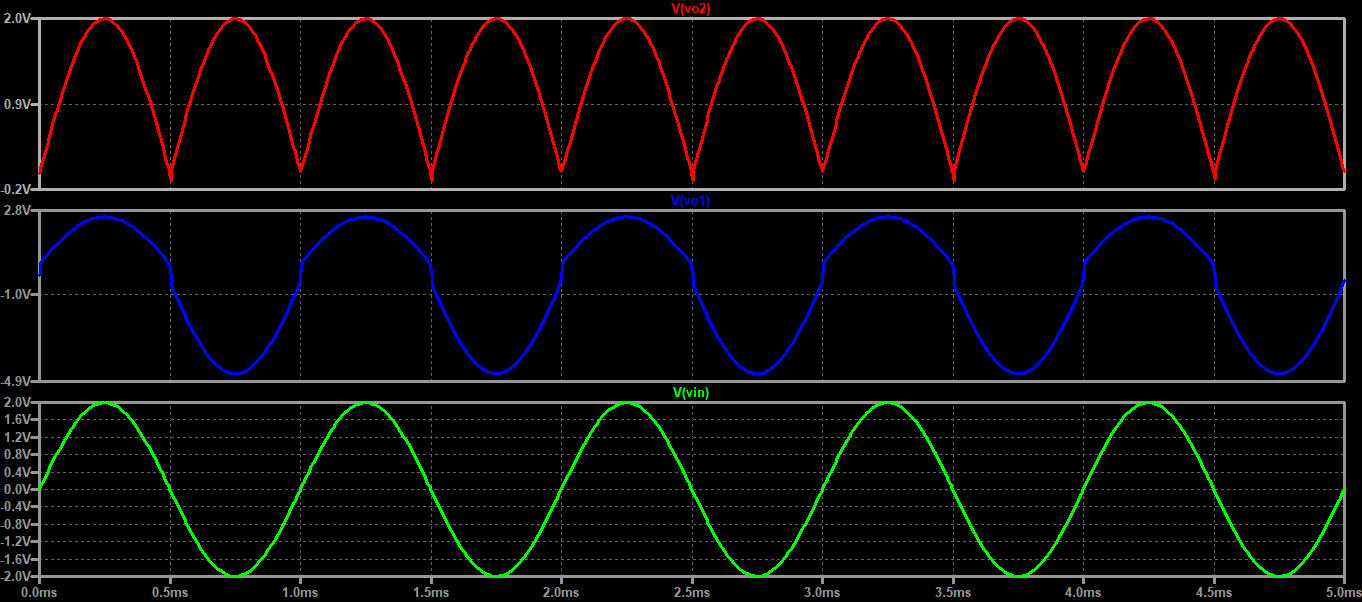
\includegraphics[width=1\textwidth]{figuras/Vo1_Vo2_Vin=2.png}
	\caption{$Vo_1$ (azul) y $Vo_2$ (rojo) con $V_{in}=2[V]$.}
\end{figure}
\begin{center}
	\begin{tabular}{| c | c |}
		\hline
		& $V_{in}= 2[V]$ \\ \hline
		$Vo_1$ 	&  	2.51 [V]	 \\
		$Vo_2$ 	& 	1.99 [V]	 \\ \hline
	\end{tabular}
\end{center}
\begin{figure}[H]
	\centering
	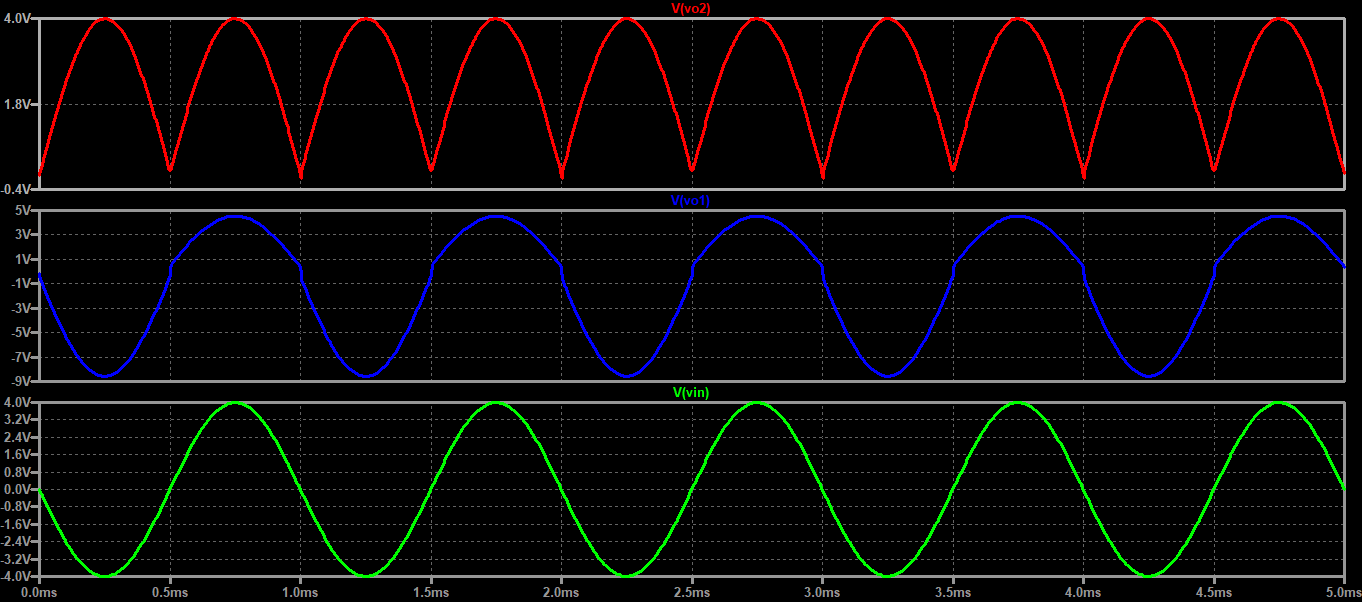
\includegraphics[width=1\textwidth]{figuras/Vo1_Vo2_Vin=-4.png}
	\caption{$Vo_1$ (azul) y $Vo_2$ (rojo) con $V_{in}=-4[V]$.}
\end{figure}
\begin{center}
	\begin{tabular}{| c | c |}
		\hline
		& $V_{in}= -4[V]$ \\ \hline
		$Vo_1$ 	&  	-8.57 [V]	 \\
		$Vo_2$ 	& 	 3.99 [V]	 \\ \hline
	\end{tabular}
\end{center}
\begin{figure}[H]
	\centering
	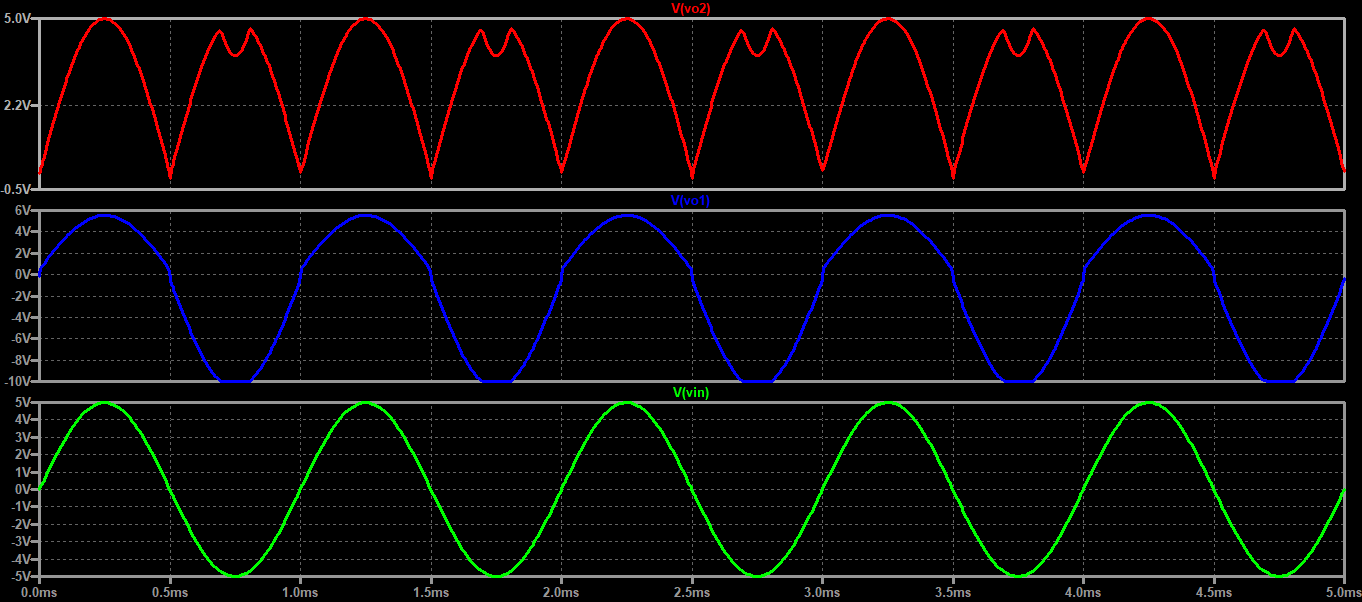
\includegraphics[width=1\textwidth]{figuras/Vo1_Vo2_Vin=5.png}
	\caption{$Vo_1$ (azul) y $Vo_2$ (rojo) con $V_{in}=5[V]$.}
\end{figure}
\begin{center}
	\begin{tabular}{| c | c |}
		\hline
		& $V_{in}= 5[V]$ \\ \hline
		$Vo_1$ 	&  	5.54 [V] 	 \\
		$Vo_2$ 	& 	4.98 [V]	 \\ \hline
	\end{tabular}
\end{center}
Como se observa para los diferentes valores de probados en el rango de -4[V] y 4[V] la señal fue rectificada correctamente. Sin embargo para valores fuera de ese rango, la salida comienza a distorsionarse debido a que la salida del primer AO comienza a saturarse debido a las alinealidades nombradas anteriormente.
